\usetikzlibrary{calc}
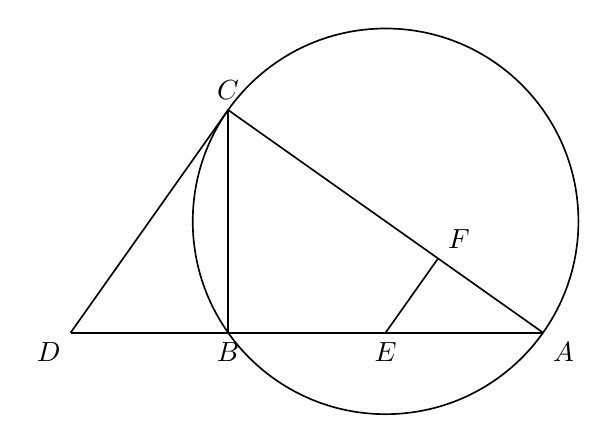
\begin{tikzpicture}[x=1cm,y=1cm,line width=.6pt,font=\normalsize]
\coordinate (O) at (2,1.414);
\coordinate (D) at (-2,0);
\coordinate (B) at (0,0);
\coordinate (E) at (2,0);
\coordinate (A) at (4,0);
\coordinate (C) at (0,2.828);
\coordinate (F) at (2.667,0.943);
\draw (O) circle[radius=2.449cm];
\draw (D)--(A);
\draw (D)--(C);
\draw (B)--(C);
\draw (C)--(A);
\draw (E)--(F);
\node[below left] at (D) {$D$};
\node[below] at (B) {$B$};
\node[below] at (E) {$E$};
\node[below right] at (A) {$A$};
\node[above] at (C) {$C$};
\node[above right] at (F) {$F$};
\end{tikzpicture}
